\documentclass[fleqn,10pt,lineno]{wlpeerj}\usepackage[]{graphicx}\usepackage[]{color}
%% maxwidth is the original width if it is less than linewidth
%% otherwise use linewidth (to make sure the graphics do not exceed the margin)
\makeatletter
\def\maxwidth{ %
  \ifdim\Gin@nat@width>\linewidth
    \linewidth
  \else
    \Gin@nat@width
  \fi
}
\makeatother

\definecolor{fgcolor}{rgb}{0.345, 0.345, 0.345}
\newcommand{\hlnum}[1]{\textcolor[rgb]{0.686,0.059,0.569}{#1}}%
\newcommand{\hlstr}[1]{\textcolor[rgb]{0.192,0.494,0.8}{#1}}%
\newcommand{\hlcom}[1]{\textcolor[rgb]{0.678,0.584,0.686}{\textit{#1}}}%
\newcommand{\hlopt}[1]{\textcolor[rgb]{0,0,0}{#1}}%
\newcommand{\hlstd}[1]{\textcolor[rgb]{0.345,0.345,0.345}{#1}}%
\newcommand{\hlkwa}[1]{\textcolor[rgb]{0.161,0.373,0.58}{\textbf{#1}}}%
\newcommand{\hlkwb}[1]{\textcolor[rgb]{0.69,0.353,0.396}{#1}}%
\newcommand{\hlkwc}[1]{\textcolor[rgb]{0.333,0.667,0.333}{#1}}%
\newcommand{\hlkwd}[1]{\textcolor[rgb]{0.737,0.353,0.396}{\textbf{#1}}}%
\let\hlipl\hlkwb

\usepackage{framed}
\makeatletter
\newenvironment{kframe}{%
 \def\at@end@of@kframe{}%
 \ifinner\ifhmode%
  \def\at@end@of@kframe{\end{minipage}}%
  \begin{minipage}{\columnwidth}%
 \fi\fi%
 \def\FrameCommand##1{\hskip\@totalleftmargin \hskip-\fboxsep
 \colorbox{shadecolor}{##1}\hskip-\fboxsep
     % There is no \\@totalrightmargin, so:
     \hskip-\linewidth \hskip-\@totalleftmargin \hskip\columnwidth}%
 \MakeFramed {\advance\hsize-\width
   \@totalleftmargin\z@ \linewidth\hsize
   \@setminipage}}%
 {\par\unskip\endMakeFramed%
 \at@end@of@kframe}
\makeatother

\definecolor{shadecolor}{rgb}{.97, .97, .97}
\definecolor{messagecolor}{rgb}{0, 0, 0}
\definecolor{warningcolor}{rgb}{1, 0, 1}
\definecolor{errorcolor}{rgb}{1, 0, 0}
\newenvironment{knitrout}{}{} % an empty environment to be redefined in TeX

\usepackage{alltt} % for journal submissions
\usepackage{hyperref}
% \documentclass[fleqn,10pt]{wlpeerj} % for preprint submissions

\title{Method for evaluating genomic material purity using whole genome sequencing data.}

\author[1]{Nathan D. Olson}
\author[1]{Justin Zook}
\author[1]{Jayne Morrow}
\author[1]{Nancy Lin}
\affil[1]{Material Measurement Laboratory, National Institute of Standards and Technology}

\keywords{Biodetection, Test material, Reference material, Purity, Bioinformatics}

\begin{abstract}
Dummy abstract text. 

\end{abstract}
\IfFileExists{upquote.sty}{\usepackage{upquote}}{}
\begin{document}















\flushbottom
\maketitle
\thispagestyle{empty}

\section*{Introduction}
Rapid, sensitive and accurate assays for detecting bacterial pathogens in food, water, clinical samples, and suspicious biothreats are critical to public health and safety. 
Biodetection assays must be evaluated for assay sensitivity and specificity prior to deployment and then in the hands of the user to instill confidence in the actions made based on assay results \citep{Ieven2013,International2011,EPA2004,ISO/TS2010,Guide1998,Feldsine2002}. 
Test materials are used to validate assay performance.  Test materials can be either purified cultures, genomic DNA or whole cells spiked into a matrix \citep{EPA2004,ISO/TS2010,CLSI2010}. 
Before being used to evaluate a biodetection assay, the material itself must be validated in terms of purity and identity to eliminate false positive results due to test material contaminants or false negatives due to the test material being the wrong strain \citep{CLSI2010}. 
There are a number of potential sources of microbial contaminants of test materials including the stock culture, preservation medium, and airborne and laboratory contaminants \citep{Marron2013,Shrestha2013,Tanner1998}.   

Currently polymerase chain reaction (PCR) assays are the most commonly use method for evaluating test material purity. 
Other methods to detect contaminants using whole genome sequencing datasets have been developed, but they are not currently used to evaluate test material purity.
A PCR assay was developed to analyze protist cultures. 
This assay uses endpoint PCR for prokaryotes and eukaryotes with template dilutions \citep{Marron2013}. 
The benefit to PCR-based approaches is that they can be cost effective and fast if an applicable protocol exists. 
Another PCR based assay was used to evaluate the purity of cyanobacterial cultures \citep{heck2016evaluating}.
While PCR assays can detect low levels of contaminants, this approach does not easily scale to multiple contaminants and test materials. 
More importantly, PCR assays can only target specific contaminants, which biases the purity assessment to known potential contaminants.
The bioinformatics tools developed to identify genomic contaminants in metagenomic datasets, which include sequencing data from all organisms in a sample, can also be used to evaluate test material purity. 
For example DeconSeq \citep{Schmieder2011} and a similar method QC-Chain \citep{Zhou2013} were developed to identify contaminants based on analysis of 16S ribosomal ribonucleic acid (rRNA) gene sequences or comparison of a subset of reads to a reference database using Basic Local Alignment Search Tool (BLAST). 
Metagonomic-based methods are ideally able to identify contaminants without any prior knowledge or assumptions regarding the identity of the organism(s). 
However, methods based on 16S rRNA gene identification have limited resolution, as 16S rRNA sequences can only provide genus level taxonomic resolution at best. 
The benefit to using metagenomic tools developed for 16S rRNA is that prior knowledge of the identity of the contaminant is not required; however, this method is unable to identify contaminants to the species level or higher.   

Another approach to evaluating test material purity is through shotgun whole genome sequencing, i.e.,  sequence all DNA in a purportedly single organism sample. 
There are a number of metagenomic read classification algorithms developed to determine the taxonomic composition of a sequence dataset of unknown composition. 
These algorithms tend to use one of three primary strategies for taxonomic assignment. 
The first method consist of aligning reads to a reference database that contains assemblies of microbial genomes \citep{buchfink2015fast, Francis2013}. 
This approach, while exaustive, is computationally expensive. 
The second type of method focuses on marker genes, genes common to different phylogenetic groups, which reduces the computational cost \citep{segata2012metagenomic, liu2011accurate}. 
The disadvantage of using only marker genes is that information required to discriminate closely related genomes may not be present in the marker genes.
The third method uses a $k$-mer based approach, where taxonomic composition is determined based the abundance of DNA sequences of length $k$ in the sequence dataset and a reference database \citep{ounit2015clark, menzel2016fast, wood2014kraken}. 

In this work, we present the results of a proof of concept study to measure the purity of single organism test materials using whole genome sequencing data combined with a metagenomic read classification algorithm. 
We choose to use \textit{Pathoscope}, a method that aligns sequences to a database of genome assemblies. 
It was developed to detect pathogens and identify strains using whole genome sequencing data \citep{Francis2013}. 
\textit{Pathoscope} benefits from the large sample size obtained using all sequence data for higher sensitivity (compared to marker gene based methods) and leverages algorithmic advances for whole genome sequence mapping. 
We will first present the specificity of the method using simulated data for single organisms. 
Then, we evaluate sensitivity of the method using simulated contaminanted test material datasets.  


\section*{Methods}
Simulated whole gnome sequence data was used to evaluat the suitability of using whole genome sequence data and metagenomic taxonomic classification methods for validating test material purity. 
Simulated data from single genomes was used to assess method specificity. 
To assess method sensitivity, contaminant datasets comprised of pairwise combinations of single genomes spiked with a defined proportion of contaminant reads, reads simulated from a different genome.  

To best approximate real sequencing data reads with simulated using empirically determined error model and insert size distributions. 
The whole genome sequencing data was simulated using the ART sequencing read simulator as the algorithm using an empirical sequencing error model \citep{Huang2012}. 
Reads were simulated with ART simulator using the Illumina MiSeq error model for 2 $\times$ 230 base pair paired end reads with an insert size of 690 $\pm$ 10 base pairs(average $\pm$ standard deviation) and 20 X mean coverage for each strain. 
The insert size parameters were defined based on the observed average and standard deviation insert size of the NIST RM8375-MG002 MiSeq sequencing data \citep{olson2016pepr}.

The taxonomic composition of simulated datasest was assessed using the Pathoscope metagenomic taxonomic classifier \citep{Francis2013}. 
This method was selected as it combines the use of a large reference database reducing potential biases due to contaminant sequences not present in the database and efficient whole genome read mapping algorithms. 
This method uses an expectation maximization algorithm where the sequence data are first mapped to a database comprised of all sequence data in the Genbank nt database. 
Then, through an iterative process, it re-assigns ambiguously mapped reads based on the proportion of reads mapped unambigously to individual taxa in the database. 
The PathoScope 2.0 taxonomic read classification pipeline has three steps; (1) PathoQC - read quality filtering and trimming using the PRINSEQ algorithm \citep{schmieder2011quality}, (2) PathoMap - mapping reads to a reference database using the bowtie2 algorithm \citep{Langmead2012}, (3) PathoID - expectation-maximization classification algorithm. 
The annotated Genbank nt database provided by the PathoScope developers was used as the reference database (\url{ftp://pathoscope.bumc.bu.edu/data/nt\_ti.fa.gz}).

\subsection*{Single Genome - Baseline Assessment}
Method specificity was first assessed to characterize the baseline accuracy of the read classifier.
Method specificity was defined as the proportion of reads in a single organism simulated dataset incorrectly assigned to a taxonomy different from the test material taxonomy. 
Sequence data was simulated for 406 strains, from 9 genera (Table \ref{tab:single_org}). 
We will refer to the genome used to generate the reads as the target genome. 
The genomes included in the simulation study were limited to the number of closed genomes in the Genbank database (\url{http://www.ncbi.nlm.nih.gov/genbank/}, accessed 10/18/2013) belonging to the genera of interest (Table \ref{tab:single_org}). 
Due to the large number of closed genomes from the genera \textit{Bacillus}, \textit{Escherichia}, and \textit{Salmonella}, these genera were limited to the species \textit{Bacillus cereus}, \textit{Escherichia coli}, and \textit{Salmonella enterica}.
The taxononomic heirarchy for the target genome and simulated read assignment match levels were determined using the R package \citep{TaxizeArticle,TaxizeManual}. 

\subsection*{Simulated Contaminants}
Method sensitivity was assessed using simulated contaminated datasets to evaluate at how well the method is able to detect genomic contaminants at a range of contaminat concentrations. 
Representative genomes for 8 of the 9 genus were used to generate the simulated contaminant datasets (Table \ref{tab:contam_table}). 
An \textit{Escherichia coli} strain was selected as a representative of both  and \textit{Shigella} as the genus \textit{Shigella} phylogenetically resides within the species \textit{Eschericha coli} \citep{lan2002escherichia}. 
For each pairwise combination of representative genomes the simulated contaminant dataset was comprised of a randomly selected subset of reads from the target and contaminant simulated single genome sequence dataset. 
The simulated datasets were subsampled at defined proportions with $p$ representing the proportion of reads from the contaminant single genome dataset subsampled and $1-p$ the proportion of reads from the target genome simulated dataset. 
A 10 fold range of contaminant proportions were simulated with $p$ ranging from $0.1$ to $10^{-8}$, resulting in 512 simulated contaminant datasets. 
This approach simulates the proportions of cells in a test material and not the amount of DNA, assuming unbiased DNA extraction. 
To generate the simulated contaminant datasets single organism simulated datasets were first generated for the 8 representative genomes using the same methods as used in the first part of the study. 
The resulting simulated sequencing data was first processed using PathoQC and PathoMap steps in the PathoScope pipeline. 
The output from the PathoMap step (sam file, sequence alignment file \url{https://samtools.github.io/hts-specs/SAMv1.pdf}) for the target and contaminant datasets were subsampled and combined and the resulting sam file was processed by PathoID, the third step in the PathoScope pipeline.
Subsampling the sam files instead of the simulated sequence files greatly reduces the computational cost of the analysis as the simulated reads were only processed by the first two steps in PathoScope pipeline rather then for every simulated contaminant dataset. 


\subsection*{Bioinformatic Pipeline}
To facilitate repeatabiliy and transparency, a Docker (\url{www.docker.com}) container is available with installed pipeline dependencies (\url{www.registry.hub.docker.com/u/natedolson/docker-pathoscope/}). 
The script used to run the simulations are available at \url{https://github.com/nate-d-olson/genomic_purity}. 
Additionally, seeds number for the random number generator was randomly assigned and recorded for each dataset so that the same simulated datasets could be regenerated.
Pathoscope results were processed using the statistical programing language R \citep{R}, and intermediate analysis and data summaries were organized using ProjectTemplate \citep{ProjectTemplate} and archived in a github repository (\url{https://github.com/nate-d-olson/genomic_purity_analysis}) along with the source file for this manuscript.

\section*{Results and Discussion}

\subsection*{Single Genome - Baselines Assessment}

Simulated sequence data from individual isolates was used to assess the genomic purity assessment method specificity. 
True negatives (TNs) are reads assigned to the target genome's species, genus, family, ect., depending on the match stringency, and false positives (FPs) are reads incorrectly assigned to a different species, genus, family, ect., and specificity = TN/(FP+TN). 
Here we use specificity as a measure of the ability of the method to correctly assign reads to the taxonomy of the genome the sequencing reads were simulated from, the target genome. 
Method specificity was evaluated by characterizing the read assignment results based on the level of agreement between the genome and assigned taxonomy (Fig. \ref{fig:single_org_cum}). 
Overall high proportion of matches at species and genus level. 
Some genus have low specificity at the species and genus levels.  
For \textit{Shigella} most likely due to matches with \textit{Escherichia} (Fig. \ref{fig:shigella_ec_cum}). 
The cumulative match proportions do not always reach 1.00, for example \textit{Staphylococcus} genomes. 
This might be due to exclusion of unclassified and unknown matches (NCBI taxid 12908 and 0 respectively) from match level analysis.

% latex table generated in R 3.3.1 by xtable 1.8-2 package
% Fri Sep  2 14:45:32 2016
\begin{table}[ht]
\centering
\begin{tabular}{lrl}
  \hline
Genus & N & Genome Size (Mb) \\ 
  \hline
\textit{Bacillus} &  76 & 5.05 (3.07-7.59) \\ 
  \textit{Escherichia} &  62 & 5.11 (3.98-5.86) \\ 
  \textit{Pseudomonas} &  57 & 6.18 (4.17-7.01) \\ 
  \textit{Staphylococcus} &  49 & 2.82 (2.69-3.08) \\ 
  \textit{Salmonella} &  44 & 4.88 (4.46-5.27) \\ 
  \textit{Listeria} &  39 & 2.97 (2.78-3.11) \\ 
  \textit{Clostridium} &  32 & 4.02 (2.55-6.67) \\ 
  \textit{Yersinia} &  19 & 4.73 (4.62-4.94) \\ 
  \textit{Francisella} &  18 & 1.89 (1.85-2.05) \\ 
  \textit{Shigella} &  10 & 4.74 (4.48-5.22) \\ 
   \hline
\end{tabular}
\caption{Breakdown of the number of genomes by genus used to generate single genome simultated datasets. N indicates the number of genomes, and Genome Size is presented as the median and range (minimum to maximum) genome size} 
\label{tab:single_org}
\end{table}


\begin{knitrout}
\definecolor{shadecolor}{rgb}{0.969, 0.969, 0.969}\color{fgcolor}\begin{figure}

{\centering 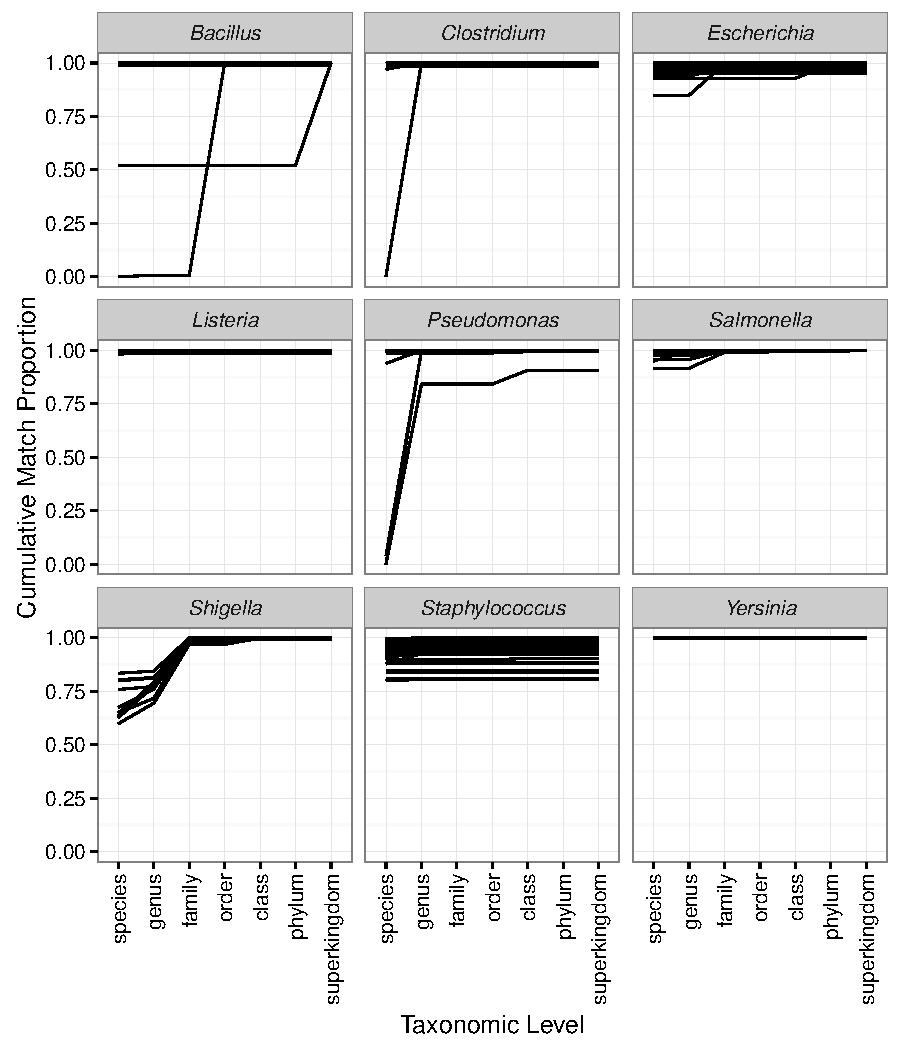
\includegraphics[width=\maxwidth]{figure/single_org_cum-1} 

}

\caption[Cumulative taxonomic match results for genomic purity assessments of simulated sequence data from single genomes]{Cumulative taxonomic match results for genomic purity assessments of simulated sequence data from single genomes.  Each line represents the cumulative proportion of simulated reads with taxonomic assignments matching at or above the specified taxonomic level. Genomes are grouped by genus.}\label{fig:single_org_cum}
\end{figure}


\end{knitrout}


\begin{knitrout}
\definecolor{shadecolor}{rgb}{0.969, 0.969, 0.969}\color{fgcolor}\begin{figure}

{\centering 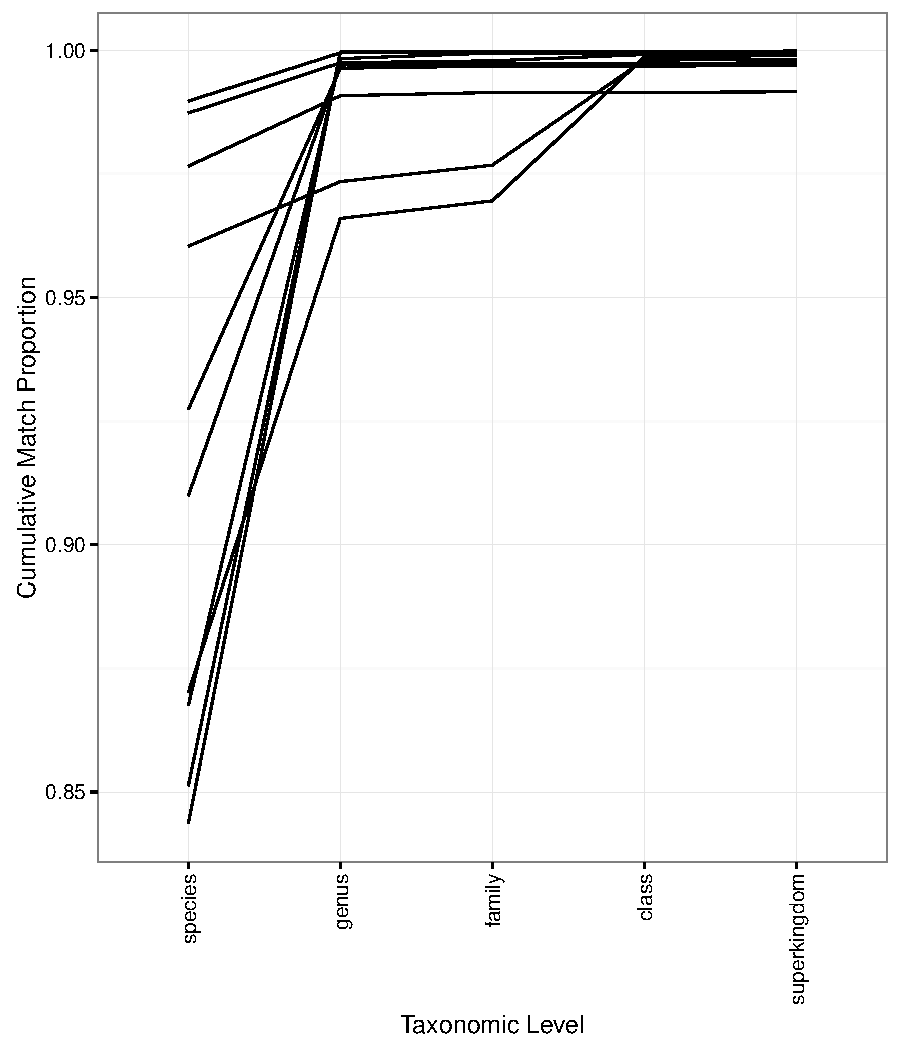
\includegraphics[width=\maxwidth]{figure/shigella_ec_cum-1} 

}

\caption{Cumulative taxonomic match results for genomic purity assessment for \textit{Shigella} considering matches to \textit{E. coli} as species level matches.  Each line represents the cumulative proportion of simulated reads with taxonomic assignments matching at or above the specified taxonomic level. Genomes are grouped by genus.}\label{fig:shigella_ec_cum}
\end{figure}


\end{knitrout}

Most of the genera had genus level or higher match proportions excluding a few outliers (Fig. \ref{fig:single_genus}). 
\textit{Escherichia}, \textit{Shigella}, and \textit{Staphylococcus} are notable exceptions. 
As discussed previously the taxonomic ambiguities for \textit{Shigella} and \textit{Escherichia} are responsible for the overall lower genus level match proportions. Another example of low genus level matches is the \textit{Bacillus} genome with genus match proportion close to zero, \textit{Bacillus infantis} string NRRL B 14911. While the \textit{B. infantis} strain was originally classified as \textit{Bacillus} the species is phylogenetically distinct from other members of the genus \citep{ko2006bacillus}.
It is important to consider the strain and genome being characterized, as taxonomic ambiguities (e.g. \textit{Shigella} and \textit{Escherichia}) can lead to lower than expected specificity and the identification of false positive contaminants.  


\begin{knitrout}
\definecolor{shadecolor}{rgb}{0.969, 0.969, 0.969}\color{fgcolor}\begin{figure}
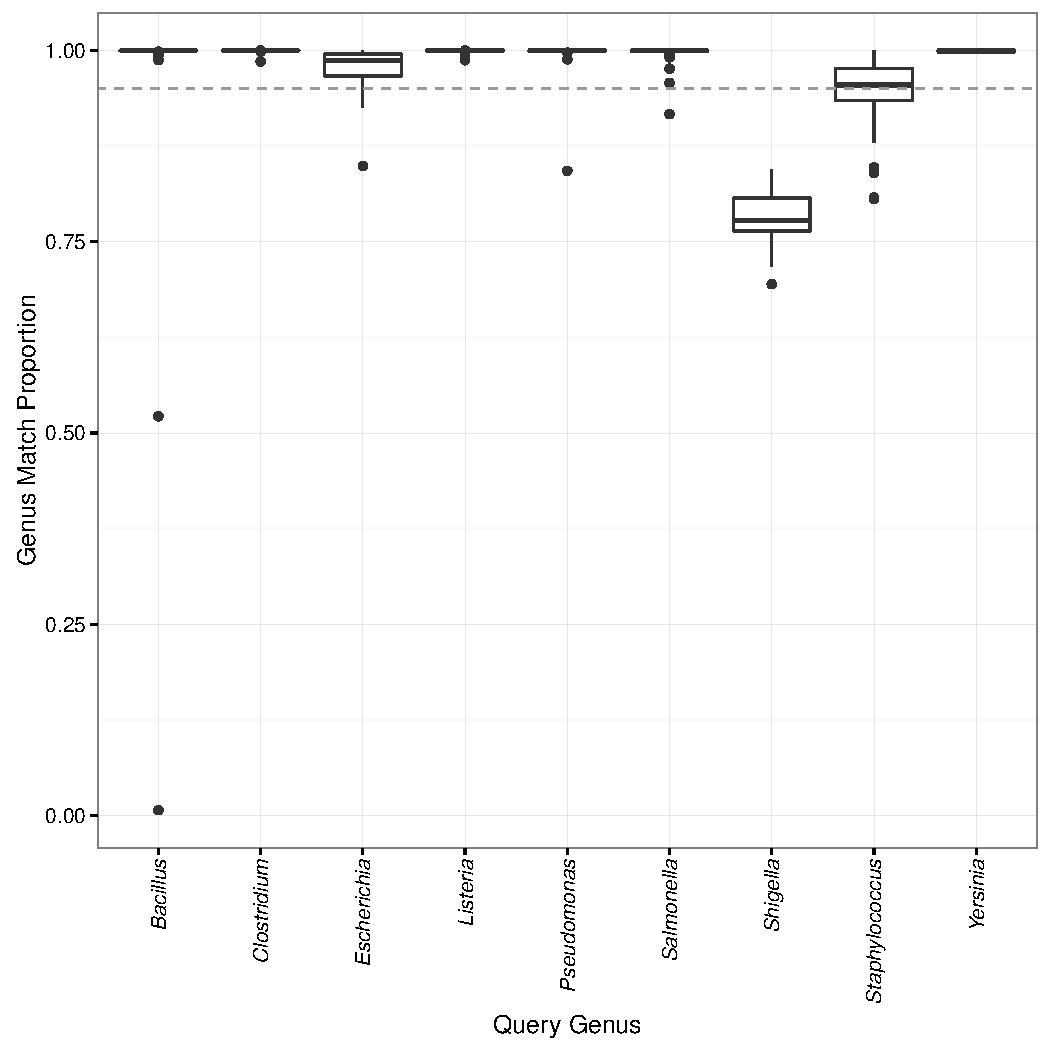
\includegraphics[width=\maxwidth]{figure/single_genus-1} \caption[Distribution of the proportion of reads assigned to the source genome at or above the genus level]{Distribution of the proportion of reads assigned to the source genome at or above the genus level. Horizontal grey line highlights a match proportion of 0.95. Boxplots hinges represent the 25th and 75th percentiles, line through box represent is the median, whiskers are the 95\% confidence interval, and the black dots are outliers.}\label{fig:single_genus}
\end{figure}


\end{knitrout}

\subsection*{Simulated Contaminants}
To evaluate genomic purity assessment methods we generated simulated contaminant datasets as pairwise combinations of representative genomes from 8 of the genera used in the specificity section of the study (Table \ref{tab:contam_table}). 
Due to the overall high proportion of reads matched to the correct genome in the method specificity study, the simulated contaminant datasets were evaluated at the genus level for sensitivity. 
For all of the genomes selected for the sensitivity study, the proportion of simulated reads that matched at species level or higher was 0.98 (Table \ref{tab:contam_table}).  

% latex table generated in R 3.3.1 by xtable 1.8-2 package
% Fri Sep  2 14:45:33 2016
\begin{table}[ht]
\centering
\scalebox{0.65}{
\begin{tabular}{lrllll}
  \hline
Representative Strain & Species & C Mb & C Acc & P Mb & P Acc \\ 
  \hline
Bacillus anthracis str. Ames & 1.00 & 5.23 & AE016879.1 &  &  \\ 
  Clostridium botulinum A str. Hall & 1.00 & 3.76 & CP000727.1 &  &  \\ 
  Escherichia coli O157:H7 str. EC4115 & 0.98 & 5.57 & CP001164.1 & 0.13 & CP001163.1, CP001165.1 \\ 
  Francisella tularensis subsp. tularensis SCHU S4 & 1.00 & 1.89 & AJ749949.2 &  &  \\ 
  Pseudomonas aeruginosa PAO1 & 1.00 & 6.26 & AE004091.2 &  &  \\ 
  Salmonella enterica subsp. enterica serovar Typhimurium str. D23580 & 1.00 & 4.88 & FN424405.1 &  &  \\ 
  Staphylococcus aureus subsp. aureus ED133 & 0.98 & 2.83 & CP001996.1 &  &  \\ 
  Yersinia pestis CO92 & 1.00 & 4.65 & AL590842.1 & 0.18 & AL109969.1, AL117189.1, AL117211.1 \\ 
   \hline
\end{tabular}
}
\caption{Representative strains used in simulated contaminant datasets. Species indicates the proportion of simulated reads assigned to the correct taxa at the species level or higher. DNA size (Mb) and Genbank accession numbers (Acc) are indicated for chromosomes (C) and plasmids (P). Escherichia coli O157:H7 str. EC4115 and Yersinia pestis CO92 have two and three plasmids respectively.} 
\label{tab:contam_table}
\end{table}


To evaluate sensitivity, we plot the proportion of reads assigned to the contaminant genus or species versus the proportion of reads simulated from the contaminating genome. 
While the proportion of contaminant reads in the simulated datasets was not equal to the defined contaminant proportion, the proportion of reads assigned to the contaminant genus was comparable to the expected proportion (Fig. \ref{fig:contam_min}). 
This was especially true for datasets containing mixtures of \textit{B. anthracis}, \textit{Y. pestis}, \textit{E. coli}, and \textit{S. enteria} as they had similar sized genomes (Table \ref{tab:contam_table}). 
Three contaminants were detected when spiked in at contaminant proportions of $10^{-8}$, \textit{B. anthracis} in \textit{E. coli} as well \textit{S. enteria} and \textit{E. coli} in \textit{Y. pestis}. 
Interestingly the proportion of assigned reads did not decrease with decreasing contaminant proportions after $10^{-4}$. 

The lowest detectable proportion of simulated contaminant level varied by both contaminant and target genome. 
All organisms had comparable minimum contamination levels for which reads were assigned to the contaminant genome. 
Two notable exceptions are \textit{Escherichia} and \textit{Yersinia}, where \textit{Bacillus}, and \textit{Salmonella} and \textit{Escherichia} were detected at the lowest contaminant levels respectively. 
As the results are from simulated data and based on proportions of simulated reads, these values do not indicate a limit of detection for the method.

\begin{knitrout}
\definecolor{shadecolor}{rgb}{0.969, 0.969, 0.969}\color{fgcolor}\begin{figure}
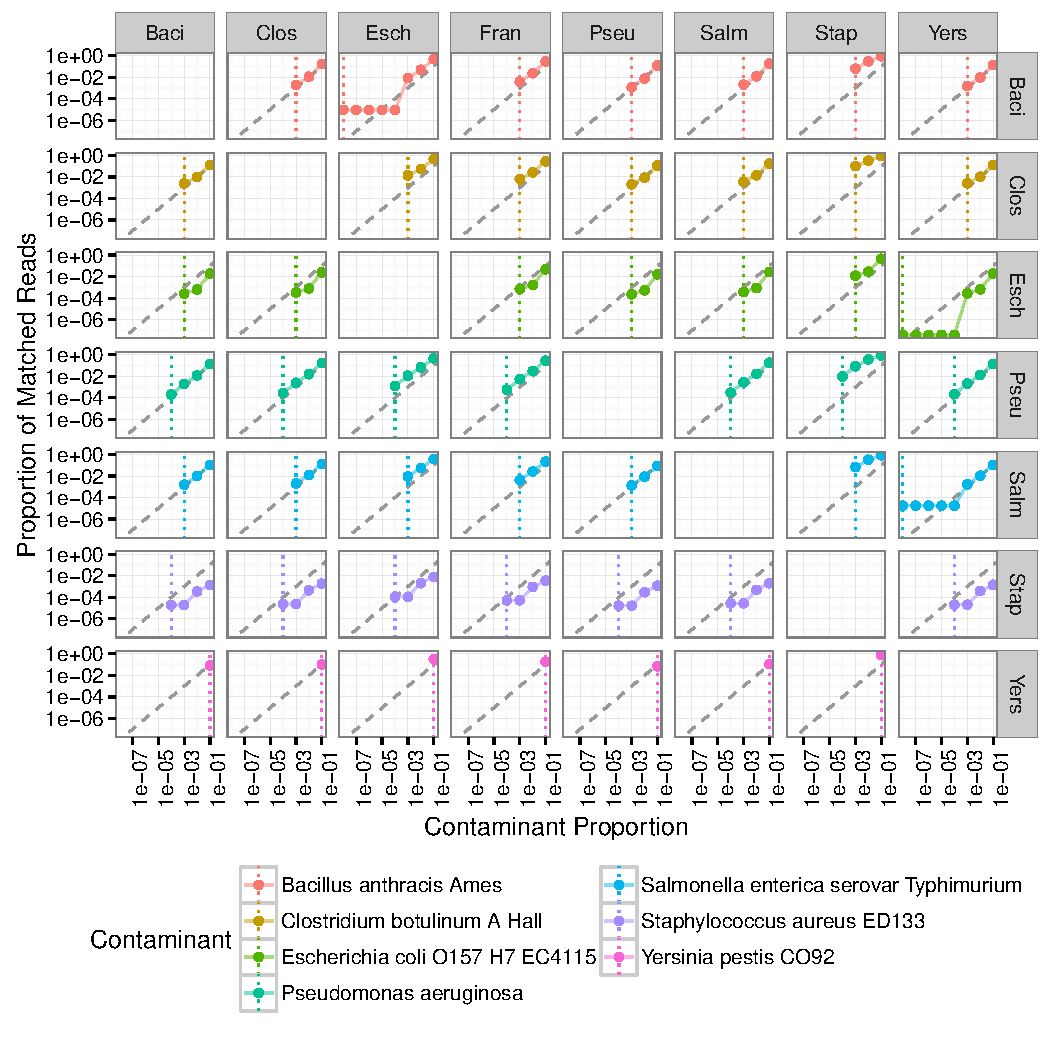
\includegraphics[width=\maxwidth]{figure/contam_min-1} \caption[Relationship between the proportion of contaminant reads simulated per dataset and the proportion of reads matched to the contaminant genus]{Relationship between the proportion of contaminant reads simulated per dataset and the proportion of reads matched to the contaminant genus.}\label{fig:contam_min}
\end{figure}


\end{knitrout}



\section*{Conclusions} 
Reference materials and strains are commonly used in basic and applied research settings. 
To ensure the validity of the conclusions drawn from the results of experiments using these materials the material genomic pruity should be evaluated. 
We have demonstrated that whole genome sequencing paired with taxonomic read classification methods are able to detect genomic contaminants at levels down to \textbf{NEED TO FILL IN} when evaluating containants as the genus level. 
While the methods used in this study produced high specificity at the genus level, other classification algorithms may result in higher specificity. 
Additionally, long read sequencing methods such as Pac Bio and Oxford Nanopore, have the potential to increase method specificity. 
The method sensitivity was dependent on the contaminant and not the target material.
This is due to the method used to generate the simulated contaminant datasets as the number of reads used in the contaminanted dataset is dependent on the genome size. 
Increasing sequencing depth is likely to result in increased sensitivity.
We have presented a proof of concept study for a novel method for evaluating test material purity. 
With the decreasing cost of whole genome sequencing this method provides a viable alternative to other commonly used methods for evaluating test material purity. 
When using whole genome sequencing in combination with metagenomic taxonomic read classifiers users should make sure to validate and optimize the methods for their specific use case. 
Validation and optimization would include selection of the appropriate database, evaluation of method sensitivity and specificity in a manner similar to what was presented here, as well as evaluation of different taxonomic classification algorithms.
\newpage

\section*{Acknowledgments}

The authors would like to thanks Dr. Steven Lund for his assistance in developing the study. 
The Department of Homeland Security (DHS) Science and Technology Directorate supported this work under the Interagency Agreement HSHQPM-12-X-00078 with the National Institute of Standards and Technology (NIST). 
Opinions expressed in this paper are the authors’ and do not necessarily reflect the policies and views of DHS,  NIST, or affiliated venues. 
Certain commercial equipment, instruments, or materials are identified in this paper in order to specify the experimental procedure adequately. 
Such identification is not intended to imply recommendations or endorsement by NIST, 
nor is it intended to imply that the materials or equipment identified are necessarily the best available for the purpose. 
Official contribution of NIST; not subject to copyrights in USA.

\bibliography{genomic_purity}

\end{document}
